% $Id: template.tex 11 2007-04-03 22:25:53Z jpeltier $

\documentclass{vgtc}                          % final (conference style)
%\documentclass[review]{vgtc}                 % review
%\documentclass[widereview]{vgtc}             % wide-spaced review
%\documentclass[preprint]{vgtc}               % preprint
%\documentclass[electronic]{vgtc}             % electronic version

%% Uncomment one of the lines above depending on where your paper is
%% in the conference process. ``review'' and ``widereview'' are for review
%% submission, ``preprint'' is for pre-publication, and the final version
%% doesn't use a specific qualifier. Further, ``electronic'' includes
%% hyperreferences for more convenient online viewing.

%% Please use one of the ``review'' options in combination with the
%% assigned online id (see below) ONLY if your paper uses a double blind
%% review process. Some conferences, like IEEE Vis and InfoVis, have NOT
%% in the past.

%% Figures should be in CMYK or Grey scale format, otherwise, colour
%% shifting may occur during the printing process.

\let\ifpdf\relax

%% These three lines bring in essential packages: ``mathptmx'' for Type 1
%% typefaces, ``graphicx'' for inclusion of EPS figures. and ``times''
%% for proper handling of the times font family.

\usepackage{mathptmx}
\usepackage{graphicx}
\usepackage{times}

%% We encourage the use of mathptmx for consistent usage of times font
%% throughout the proceedings. However, if you encounter conflicts
%% with other math-related packages, you may want to disable it.

% customer packages
\usepackage{amsmath}
\usepackage{epstopdf}
\usepackage{caption}
\usepackage{subcaption}
\usepackage{multirow}
\usepackage{algorithmicx}
\usepackage{algorithm}
\usepackage{algpseudocode}

\newcommand{\vcenterbox}[1]{\begingroup\setbox0=\hbox{#1}       \parbox{\wd0}{\box0}\endgroup}

%% If you are submitting a paper to a conference for review with a double
%% blind reviewing process, please replace the value ``0'' below with your
%% OnlineID. Otherwise, you may safely leave it at ``0''.
\onlineid{114}

%% declare the category of your paper, only shown in review mode
\vgtccategory{Technique}

%% allow for this line if you want the electronic option to work properly
\vgtcinsertpkg

%% In preprint mode you may define your own headline.
%\preprinttext{To appear in an IEEE VGTC sponsored conference.}

%% Paper title.

\title{A Bayesian Approach for Probabilistic Streamline Computation in Uncertain Flows}

%% This is how authors are specified in the conference style

%% Author and Affiliation (single author).
%%\author{Roy G. Biv\thanks{e-mail: roy.g.biv@aol.com}}
%%\affiliation{\scriptsize Allied Widgets Research}

%% Author and Affiliation (multiple authors with single affiliations).
\author{Wenbin He\thanks{e-mail: he.495@osu.edu} %
\and Chun-Ming Chen\thanks{e-mail: chen.1701@osu.edu} %
\and Xiaotong Liu\thanks{e-mail: liu.1952@osu.edu}
\and Han-Wei Shen\thanks{e-mail: hwshen@cse.ohio-state.edu}}
\affiliation{\scriptsize The Ohio State University}

% %% Author and Affiliation (multiple authors with multiple affiliations)
% \author{Roy G. Biv\thanks{e-mail: roy.g.biv@aol.com}\\ %
%         \scriptsize Starbucks Research %
% \and Ed Grimley\thanks{e-mail:ed.grimley@aol.com}\\ %
%      \scriptsize Grimley Widgets, Inc. %
% \and Martha Stewart\thanks{e-mail:martha.stewart@marthastewart.com}\\ %
%      \parbox{1.4in}{\scriptsize \centering Martha Stewart Enterprises \\ Microsoft Research}}

%% A teaser figure can be included as follows, but is not recommended since
%% the space is now taken up by a full width abstract.
%\teaser{
%  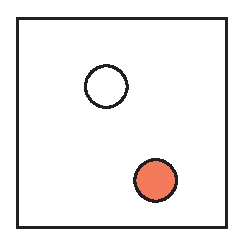
\includegraphics[width=1.5in]{sample.eps}
%  \caption{Lookit! Lookit!}
%}

%% Abstract section.
\abstract{
Streamline-based techniques play an important role in visualizing and analyzing uncertain steady vector fields. It is a challenging problem to generate accurate streamlines in uncertain vector fields due to the global uncertainty transportation. In this work, we present a novel probabilistic method for streamline computation on uncertain steady vector fields using a Bayesian framework. In our framework, a streamline is modeled as a state space model which captures the spatial coherence of integration steps and uncertainty in local distributions using the conditional prior density and the likelihood function. To approximate the posterior distribution for all the possible traces originating from a given seed position, a set of weighted samples are iteratively updated from which streamlines with higher likelihood can be derived. We qualitatively and quantitatively compare our method with alternative methods on different types of flow field data sets. Our method can generate possible streamlines with higher certainty and hence more accurate flow traces.
} % end of abstract

% %% ACM Computing Classification System (CCS).
% %% See <http://www.acm.org/class/1998/> for details.
% %% The ``\CCScat'' command takes four arguments.

% \CCScatlist{
%   \CCScat{K.6.1}{Management of Computing and Information Systems}%
% {Project and People Management}{Life Cycle};
%   \CCScat{K.7.m}{The Computing Profession}{Miscellaneous}{Ethics}
% }

%% Copyright space is enabled by default as required by guidelines.
%% It is disabled by the 'review' option or via the following command:
% \nocopyrightspace

%%%%%%%%%%%%%%%%%%%%%%%%%%%%%%%%%%%%%%%%%%%%%%%%%%%%%%%%%%%%%%%%
%%%%%%%%%%%%%%%%%%%%%% START OF THE PAPER %%%%%%%%%%%%%%%%%%%%%%
%%%%%%%%%%%%%%%%%%%%%%%%%%%%%%%%%%%%%%%%%%%%%%%%%%%%%%%%%%%%%%%%%

\begin{document}

%% The ``\maketitle'' command must be the first command after the
%% ``\begin{document}'' command. It prepares and prints the title block.

%% the only exception to this rule is the \firstsection command
\firstsection{Introduction}

\maketitle

Uncertainty is introduced in scientific data sets from various sources. As the computation power and storage capacity of modern computers continue to grow, simulations can now produce data at very high spatial and temporal resolutions, which makes it necessary to choose a representation for analysis at a reduced size. Several data reduction techniques have been introduced to solve big data problems~\cite{6378985, 7156380, conf/ldav/LiuLBP12, DBLP:conf/ldav/ThompsonLBBGPP11}, which inevitably introduce uncertainty into the resulting data. And more recently, ensembles of simulations and stochastic simulations are becoming increasingly popular, which produce data with uncertainty in nature. Further more, uncertainty may also come from errors produced by numerical simulations or instrument measurements. Hence, analyzing and visualizing uncertainty is becoming increasingly indispensable to the understanding of scientific data.

In many scientific and engineering disciplines, analysis and visualization of vector fields continue to play an important role. To date, various techniques have been developed, among which streamline based techniques play a key role in steady vector fields exploration. Although a variety of methods have been introduced to analyze and visualize uncertain vector fields, the streamline computation for uncertain vector fields is still a challenging problem. Generating streamlines that have a higher likelihood to occur in an uncertain vector field is non-trivial because the uncertainty is propagated and accumulated along the streamlines. Previously, researchers have used the Monte Carlo approach to integrate probabilistic particle traces, such as the work presented by Otto et al.~\cite{Otto10a, Otto11a}. Although the Monte Carlo method is easy to understand and implement, it suffers from several drawbacks. First, it is sensitive to local uncertainties in vector fields. When a particle passes through a highly uncertain region, the results of the trajectory estimation can be poor. Second, the spatial coherence of vector directions was not considered. As a result, the particles can change their directions abruptly along their trajectories.

In this paper, we propose a novel Bayesian approach for probabilistic particle tracing. Our approach is inspired by the following observations: Since physical phenomena often have a continuous nature, vector directions in a flow field are typically correlated in the spatial domain. Hence, the correlation between vector directions along a streamline, which is generated from such steady vector fields, should be considered. In order to take advantage of these observations, we formulate the probabilistic particle tracing problem by a state space hidden Markov model. We model the probability that a particle will encounter from one vector direction to the next as the prior density to characterize the correlation between vector directions of adjacent integration steps, and use the observation density from the data to characterize the uncertainty of local vector directions. Based on the Bayesian model, we compute the posterior distribution of streamlines to estimate the trajectories that are more likely for a particle to follow. Since it is unlikely that the prior or observation densities derived from real world data sets are Gaussian, we make use of the particle filtering~\cite{doucet2001sequential} technique in this work. In the end, we render the estimated uncertain streamline bundles and search for the most likely trajectory within. The contribution of the work is that we introduce a Bayesian model to improve the quality of uncertain particle tracing. Through experiments on different types of vector fields, the proposed method produces streamline bundles of higher likelihood and hence more accurate paths.

%% \section{Introduction}

\section{Related Work}

In this section, we first review previous works related to uncertain flow visualization. Then we give the background and related works about particle filtering.

\textbf{Uncertain Flow Visualization.} One group of the methods focused on visualizing the local uncertainty. This class of algorithms treated uncertainty within the flow field as a local phenomenon. Glyph-based approaches were discussed in~\cite{citeulike:4002316, conf/visualization/LodhaPSW96}, and texture-based methods were proposed in~\cite{botchen:2006:IVUF, 10.1109/VIS.2005.97}. In~\cite{zuk:2008:UBVF}, a method was introduced to visualize uncertainty in bidirectional vector fields. Edge Map was proposed by \cite{10.1109/TVCG.2011.265} to visualize flow fields with quantified spatial and temporal errors. \cite{conf/visualization/SandersonJK04} presented a reaction-diffusion model to visualize the uncertainty. There exist approaches that were designed to visualize global uncertainty which is transported within the flow, such as topology based approaches presented in~\cite{Otto10a, Otto11a}. However, none of the approaches above focused on solving the uncertain particle tracing problem, which is still one of the most popular flow visualization techniques.

\textbf{Particle Filtering.} In this work, we make use of a well-known feature tracking framework called particle filtering~\cite{doucet2001sequential}, which has been successfully used in computer vision and medical image analysis. Many problems in these fields involve tracking unknown quantities from some given observations, such as road tracking and fiber tracking. Generally, prior knowledge has been modeled for these phenomenon and Bayesian models can be formulated with prior distributions for the target of interest and likelihood functions for the observations. Then the tracking problem can be solved based on posterior distributions. The particle filter provides a convenient and attractive approach to evaluate the posterior distributions without any constraint about the data. It has been developed over decades and been successfully applied to solve many real world problems. \cite{bb69534, journals/pami/GemanJ96} applied this approach for human body gestures and road tracking. \cite{Brun02whitematter, bjornemoMICCAI02} introduced particle filtering for probabilistic fiber tracking, which was then improved by~\cite{journals/mia/PontabryROSKD13, Zhang20095}. In visualization community, Zhang et al. also applied this method for tracking the movement of dynamic voxels~\cite{Zhao2012}.


\section{Probabilistic Particle Tracing Model}

In order to analyze the uncertain flow field by particle tracing, in this section we introduce our probability-based particle tracing model. First, we describe the global modeling of streamlines and how to estimate the trace distributions for a given uncertain data. Then local distributions used by the global model are detailed.

\subsection{Global Modeling}

A single streamline $L$ originating from position ${x_0}$ can be modeled as $L = \{ {x_0},{x_1},...,{x_n}\} = {x_{0:n}}$, where $x_t$ refers to a position in $\mathrm{R}^d$. As mentioned by Otto et al. in~\cite{Otto10a, Otto11a}, conventional streamline integration methods such as RK4 are not well defined for uncertain vector fields, since there is no unique vector direction at a location ${x_t}$. Therefore, as with most previous methods~\cite{Otto10a, Otto11a}, we make use of the Euler integration model in this paper:
\begin{equation}
  {x_{t + 1}} = {x_t} + {v_t}\Delta t
\end{equation}
where ${v_t}$ and $\Delta t$ refer to the vector direction and the step size at step $t$. Since we focus on generating streamlines from steady vector fields in this work, it is safe to ignore the magnitude of the vectors. And if we set the step size $\Delta t$ as a constant, we can represent the streamline by a sequence of vector directions ${L = v_{0:n}}$, since the streamline trajectory only depends on the propagation directions $v_{0:n}$.

For the uncertain vector fields, there is no unique streamline $v_{0:n}$ for a given starting point $x_0$. Let $\Omega_{x_0}$ be the set of all possible streamlines which originate from $x_0$ given the uncertain data $\mathcal{H}$, we then can define a probability density function (pdf) over the path space, which is:
\begin{equation}
  p(v_{0:n}|\mathcal{H})
\end{equation}
where $\mathcal{H}$ is the set of observations from the uncertain data along the streamline trajectory. Here, we denote the distribution obtained at the starting point $x_t$ of a vector $v_t$ as $\lambda_t=\mathcal{H}(v_t)$. By applying the Bayes theorem, the target distribution $p({v_{0:n}}|{\lambda_{0:n}})$ can be represented by the prior density $p({v_{0:n}})$ and the conditional observation density $p({\lambda_{0:n}}|{v_{0:n}})$, as:
\begin{equation}
  p({v_{0:n}}|{\lambda_{0:n}}) = \frac{{p({v_{0:n}})p({\lambda_{0:n}}|{v_{0:n}})}}{{p({\lambda_{0:n}})}}
\end{equation}
where ${p({\lambda_{0:n}})}$ is a normalizing constant for a fixed data realization, which equals to $\int {p({v_{0:n}},{\lambda_{0:n}})} d{v_{0:n}}$.

Scientific simulations commonly represent physical phenomena as continuous functions. Thus, the sequence of vector directions $v_{0:n}$ along the particle trace should be correlated. This constraint can be modeled as a conditional prior density $p({v_t}|{v_{0:t - 1}})$. In this paper, we assume the sequence $v_{0:n}$ forms a Markov chain, which means the vector direction $v_t$ only depends on the previous direction $v_{t-1}$, but not on $v_{t-2},...,v_0$; so:
\begin{equation}
  p({v_t}|{v_{0:t - 1}}) = p({v_t}|{v_{t - 1}})
\end{equation}
where $p({v_t}|{v_{t - 1}})$ denotes the probability density associated with the transition from $v_{t - 1}$ to $v_t$. Hence, the probability density for a given streamline can be formulated as:
\begin{equation}
  p({v_{0:n}}) = p({v_0})\prod\limits_{t = 1}^n {p({v_t}|{v_{t - 1}})}
\end{equation}
where $p(v_0)$ can be defined by a uniform distribution, since no prior knowledge is applied.

By measuring the observations $\lambda_{0:n}$ along a given streamline $v_{0:n}$, we can get the conditional observation density $p({\lambda_{0:n}}|v_{0:n})$, which defines a measure of how the observations match the given path. In the other word, the observation density gives how likely the distributions $\lambda_{0:n}$ will be observed if the given streamline $v_{0:n}$ actually exists in the flow field. Likewise, we assume that the observation measured at a point does not depend on any previous points in the trace, i.e.:
\begin{equation}
  p(\lambda_t|v_{0:t}) = p({\lambda_t}|{v_t})
\end{equation}
which defines the likelihood density:
\begin{equation}
  p({\lambda_{0:n}}|{v_{0:n}}) = \prod\limits_{t = 0}^n {p({\lambda_t}|{v_t})}
\end{equation}

By substituting (5) and (7) into (3), the posterior density $p({v_{0:n}}|{\lambda_{0:n}})$ can be expanded as:
\begin{equation}
  p({v_{0:n}}|{\lambda_{0:n}}) = \frac{{p({v_0})\prod\limits_{t = 1}^n {p({v_t}|{v_{t - 1}})} \prod\limits_{t = 0}^n {p({\lambda_t}|{v_t})} }}{{p({\lambda_{0:n}})}}
\end{equation}

Since $p({v_{0:n}}|{\lambda_{0:n}})$ is high-dimensional, non-standard, and only known up to a proportionality constant, which makes it infeasible to be evaluated in closed-form. Therefore, a Monte Carlo based method needs to be used to approximate the target distribution. In this case, particle filtering~\cite{doucet2001sequential} as one of Sequential Monte Carlo methods is suitable to approximate the target distribution in iterations. We first put a number of weighted particles at the seed position and update them iteratively. At each iteration, the vector directions which the particles will propagate along with are sampled from an importance function. Then the weight of each particle can be updated based on the importance sampling. Furthermore, the particles can be resampled based on their weights. In the end, a set of weighted particle tracing are obtained to represent the target posterior distribution, from which the most likely trace can be chosen by maximum a posteriori estimation (MAP) estimation.

\subsection{Local Modeling}

Based on the particle filtering algorithm, the prior density $p({v_t}|{v_{t - 1}})$, the observation density $p({\lambda_t}|{v_t})$, and an importance function need to be modeled and estimated. In this section, we will elaborate how to model and estimate these local densities in detail.

\noindent\textbf{Prior Density.} As mentioned before, prior density is used to characterize the correlation between two adjacent vector directions. In this work, a prior density which prefers to continue in the previous direction and gives decreasing probability for sharper turns is used. As presented by Zhang et al. in~\cite{Zhang20095}, the von Mises-Fisher distribution~\cite{fisher} has been selected as the prior density due to its mathematical simplicity and tractability.

For a random $d$-dimensional unit vector $v$ on the $(d-1)$-dimensional sphere, with respect to the mean direction $\mu$ and the concentration parameter $\kappa$, the probability density function of the von Mises-Fisher distribution is given by
\begin{equation}
  f_{d}(v| \mu, \kappa)=C_{d}(\kappa)\exp \left( {\kappa \mu^T v } \right)
\end{equation}
where the normalization constant $C_{d}(\kappa)\,$ is
\begin{equation}
  C_{d}(\kappa)=\frac {\kappa^{d/2-1}} {(2\pi)^{d/2}I_{d/2-1}(\kappa)} \,
\end{equation}
in which $I_{d/2-1}$ denotes the modified Bessel function of the first kind and order $d/2-1$.

The parameter $\kappa$ is used to control the concentration of the distribution around the mean direction $\mu$. Figure~\ref{fisher} gives examples of points sampled from 2-dimensional von Mises-Fisher distributions with different $\kappa$.

\begin{figure}[htb]
  \centering
  \begin{subfigure}[b]{0.16\textwidth}
    \centering
    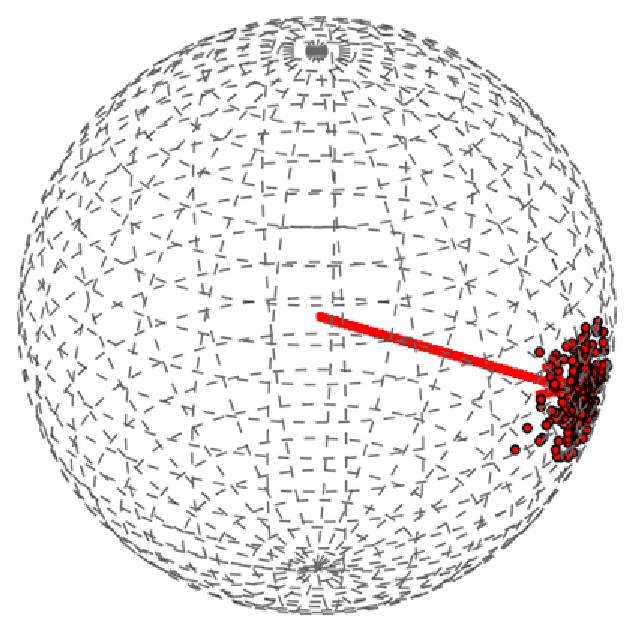
\includegraphics[width=0.8in]{../figures/vf_100.eps}
    \caption{$\kappa=100$}
  \end{subfigure}~
  \begin{subfigure}[b]{0.16\textwidth}
    \centering
    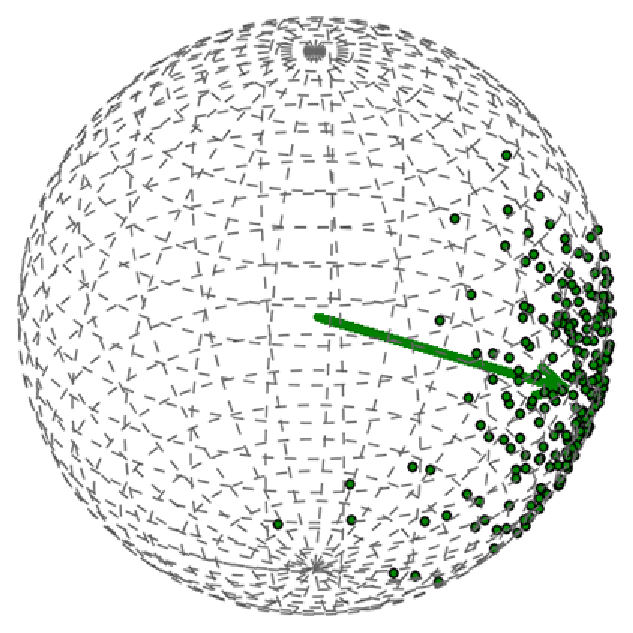
\includegraphics[width=0.8in]{../figures/vf_10.eps}
    \caption{$\kappa=10$}
  \end{subfigure}~
  \begin{subfigure}[b]{0.16\textwidth}
    \centering
    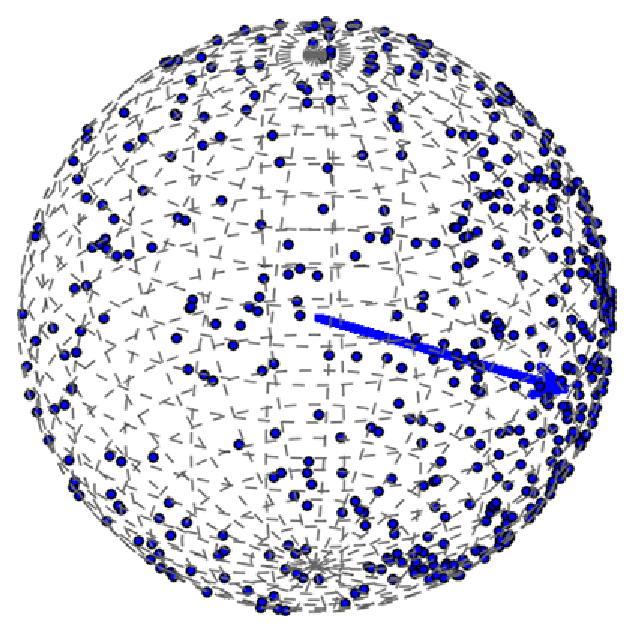
\includegraphics[width=0.8in]{../figures/vf_1.eps}
    \caption{$\kappa=1$}
  \end{subfigure}
  \caption{Points sampled from three von Mises-Fisher distributions on $2$-dimensional spheres with different value of $\kappa$. The mean directions are shown as arrows.}
  \label{fisher}
\end{figure}

In this work, the mean direction $\mu$ of the prior density is given by the previous vector direction ${v_{t - 1}}$. The concentration parameter $\kappa$ is given manually as a constant value, in this work a $\kappa = 60$ is used. For more turbulent flow fields, a larger $\kappa$ can be used.

\noindent\textbf{Observation Density.} We make use of the observation density to characterize local uncertainties, which defines a likelihood function that measures how observations match the current prior model. At step $t$, for a given vector direction $v_t$, the observation density $p({\lambda_t}|{v_t})$ is a conditional density representing how likely the observation $\lambda_t$ measured at position $x_t$ will happen based on the given vector $v_t$. According to the observation $\lambda_t$, the observation density $p({\lambda_t}|{v_t})$ is estimated based on the method presented by Friman et al. in~\cite{frimanTMI06}. We first model the observation matching perfectly to the current state $v_t$ as a distribution $\mu_t$ where the probability of $v_t$ equals to $1$. Then treat $\lambda_t$ as a histogram and let the probability $\lambda_t(i)$ of bin $i$ be an uncertain observation of $\mu_t(i)$, i.e. $\log{\mu_t(i)}=\log{\lambda_t(i)}+\epsilon$. The noise $\epsilon$ can be modeled as additive Gaussian distribution~\cite{Basser1994,Salvador05}, such as $\epsilon \sim N(0,{\sigma ^2}/{\mu _t}{(i)^2})$. Then the observation density, or the likelihood, can be written as
\begin{equation}
  p({\lambda_t}|{v_t}) = \prod\limits_{i = 0}^N {\frac{{{\mu _t}(i)}}{{\sqrt {2\pi {\sigma ^2}} }}} {e^{ - \frac{{{\mu _t}{{(i)}^2}}}{{{2\sigma ^2}}}{{(\log{{\lambda _t}(i)} - \log{{\mu _t}(i)})}^2}}}
\end{equation}

\noindent\textbf{Importance Density.} A usual approach is to use the same distribution as the prior density as the importance function, which is called bootstrap filter or condensation algorithm. However, such importance function may not be always effective, since no observation information is used. As a result, the resulting particles are often outliers of the posterior distribution. Therefore, the observation density is used to determine the $v_t$. Since it is expensive to evaluate the observation density function and there is no need to use the actual observation density as the importance density for the particle filtering method, we choose the observed distribution $\lambda_t$ as the importance density function.


\section{Results and Discussion}

We present results with different types of flow field data sets to evaluate our approach, including synthetic data and spatially aggregated data sets. To demonstrate the effectiveness of the proposed algorithm, we compared it with the Monte Carlo (MC) method, which is the general approach to stochastically trace particles in uncertain flow fields. We performed quantitative comparisons on the resulting streamlines generated by our approach and the MC method with different settings and distance measurements. We also qualitatively compare the most likely streamlines as well as the distributions of possible traces produced by our approach and the MC method by visualizing sample traces on different data sets.

\subsection{Synthetic Data}

We first evaluate the proposed algorithm on the analytical static double-gyre data set proposed by Shadden et al. in~\cite{Shadden2005271}. Gaussian noise is added into the vector field to synthesize the uncertainty. In order to quantitatively evaluate the robustness of the proposed algorithm under the influence of noise, we generate streamlines starting from regularly sampled seed positions for the certain double-gyre data set and use those streamlines as our ground truth. Then, a set of sample traces are generated by the MC method and the Bayesian approach starting from the same seed position presented above for the uncertain double-gyre data set with different noise level, which is controlled by the standard deviation $\sigma$ of the Gaussian noise. All the streamlines were generated with a step size of $0.005$ and a maximum step number of $100$. For the Monte Carlo method and the proposed algorithm, a critical parameter is the number of particles used for each seed. Indeed, more particles will give a more accurate presentation of the target distribution but will take more time to generate the results. Hence, a particle count that balances the accuracy and the computation time need to be studied. Based on~\cite{journals/mia/PontabryROSKD13}, we use $100$ particles for both of the methods in the experiments. To compare the accuracy of the resulting traces, the Hausdorff distance~\cite{Roessl:2012:TVCG} and the Mean of the closest point distance~\cite{Corouge04towardsa} between streamlines were used. Figure~\ref{gerror} gives the average of the distances presented above between the most likely streamlines generated from each method and the ground truth, with increasing $\sigma$ values for the noise in the vector field. The figure reveals that our method can produce most likely traces that are closer to the ground truth and the average of the distances increases more slowly than the MC method as the noise increases.

Besides comparing the accuracy of the most likely traces, it is also important to compare the whole distribution of possible traces generated by each method. We evaluate the accuracy of uncertain streamlines starting from a given seed position by measuring the distance between each individual trace and the ground truth, then we compute the weighted sum of all the distances. For the MC method, all traces are equally weighted. For the proposed method, the weights of the traces described above are used. Figure~\ref{gerror_r} shows that the proposed method can generate more accurate traces with less uncertainty.

\begin{figure}[!htb]
  \centering
  \begin{subfigure}[b]{0.24\textwidth}
    \centering
    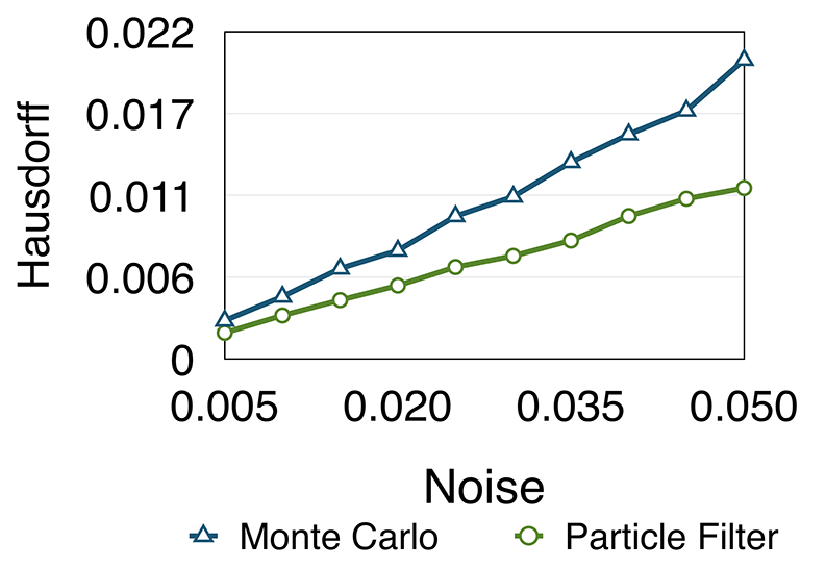
\includegraphics[height=0.8in]{../figures/doublegyre_h.eps}
  \end{subfigure}~
  \begin{subfigure}[b]{0.24\textwidth}
    \centering
    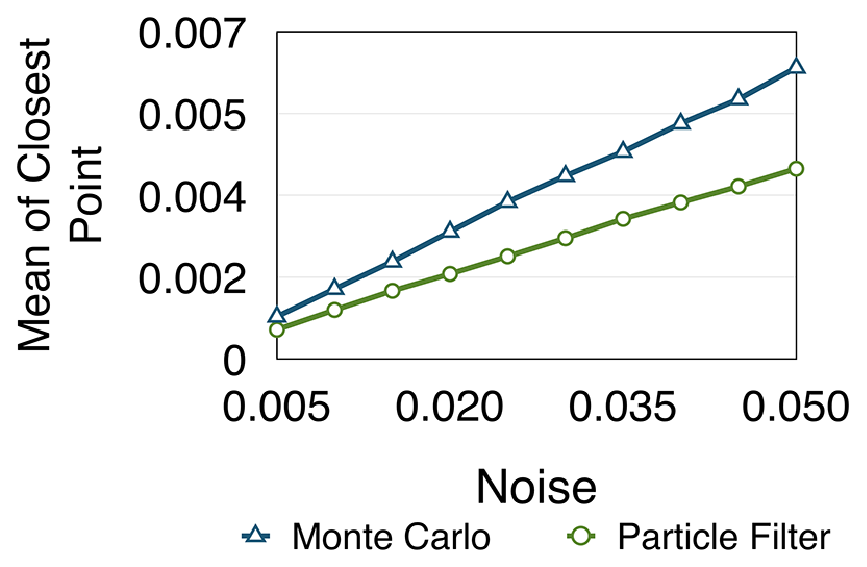
\includegraphics[height=0.8in]{../figures/doublegyre_m.eps}
  \end{subfigure}
  \caption{Comparison of the distance between the most likely traces and the ground truth for our method and the MC method.}
  \label{gerror}
\end{figure}

\begin{figure}[!htb]
  \centering
  \begin{subfigure}[b]{0.24\textwidth}
    \centering
    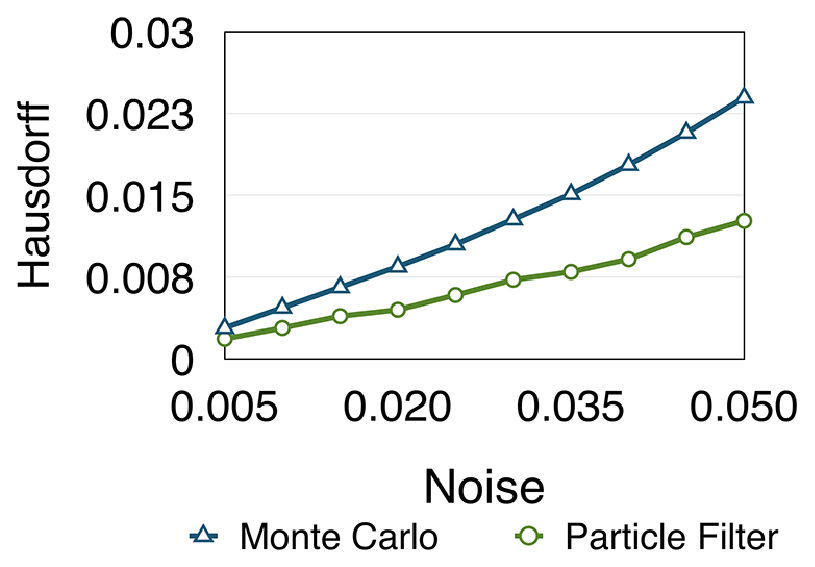
\includegraphics[height=0.8in]{../figures/doublegyre_hr.eps}
  \end{subfigure}~
  \begin{subfigure}[b]{0.24\textwidth}
    \centering
    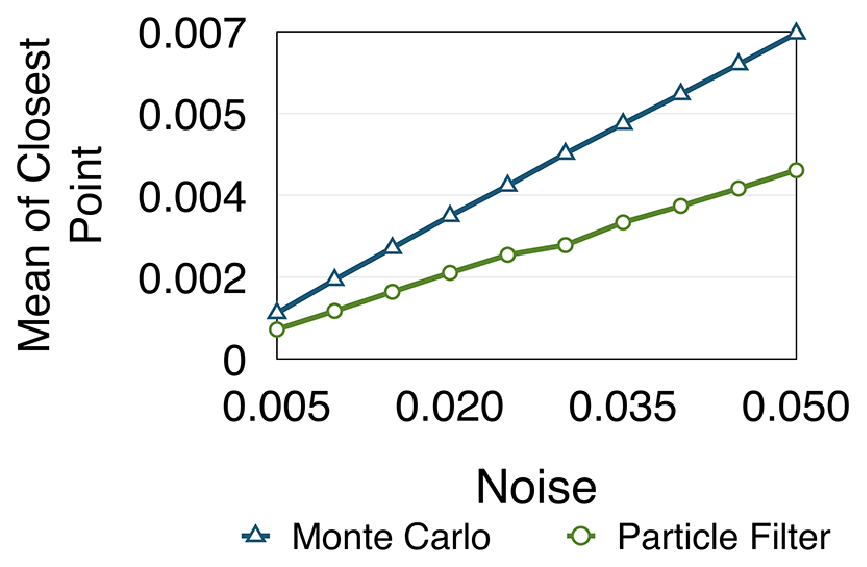
\includegraphics[height=0.8in]{../figures/doublegyre_mr.eps}
  \end{subfigure}
  \caption{Comparison of overall trace accuracy. For each method, distances of all sample traces to the ground truth are measured and summed by their weights.}
  \label{gerror_r}
\end{figure}

Figure~\ref{case_1} shows sample traces generated by the MC method and the proposed method at a given seed location in the double-gyre flow field. As we can see in the figure, our method can generate more concentrated traces which are also closer to the ground truth compared with the MC method. The most likely trace generated by the proposed method is also closer to the ground truth, as shown in~\ref{case_1} (c).

\begin{figure}[!htb]
   \centering
  \small
  (a) \vcenterbox{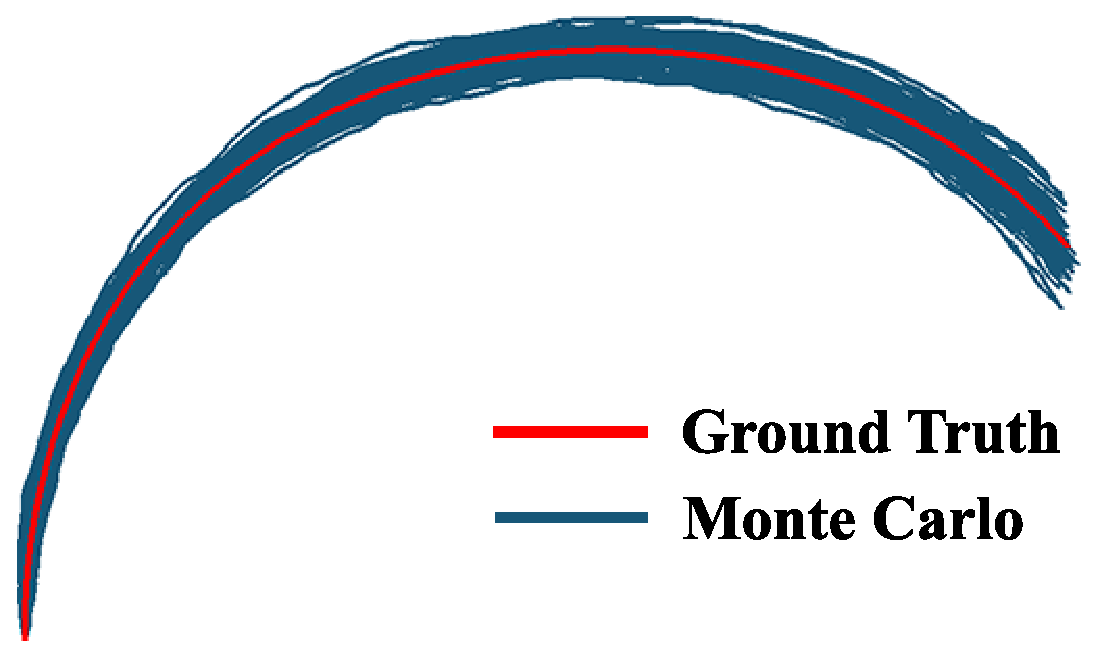
\includegraphics[height=0.5in]{../figures/double_gyre_mc35.eps} } \hfill
  (b) \vcenterbox{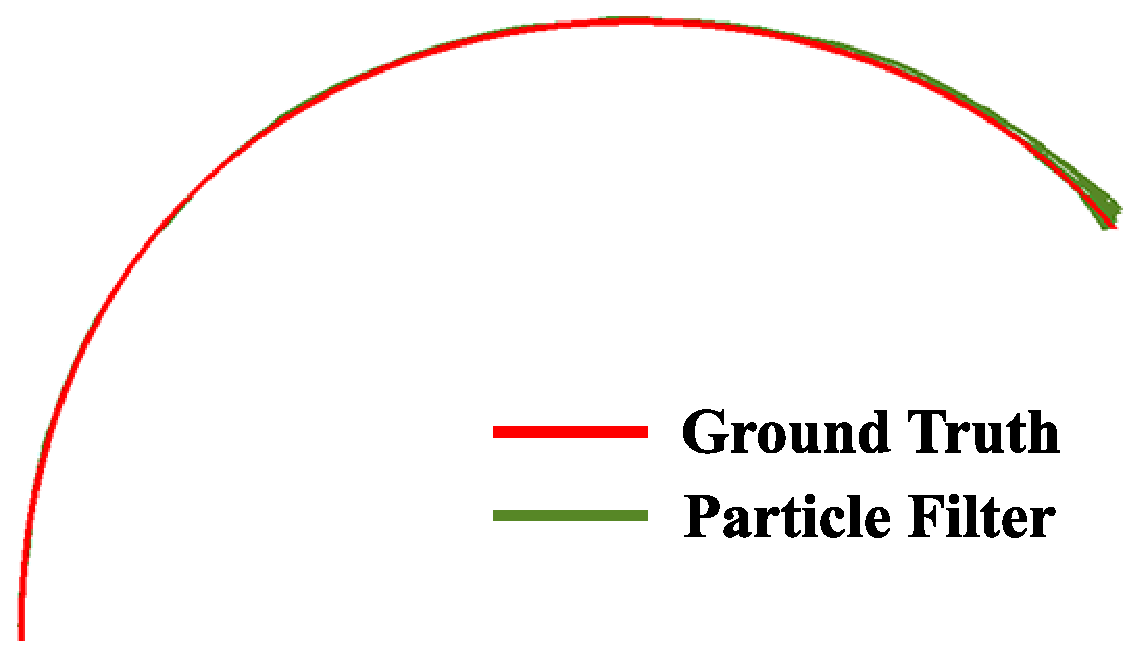
\includegraphics[height=0.5in]{../figures/double_gyre_smc35.eps} } \hfill
  (c) \vcenterbox{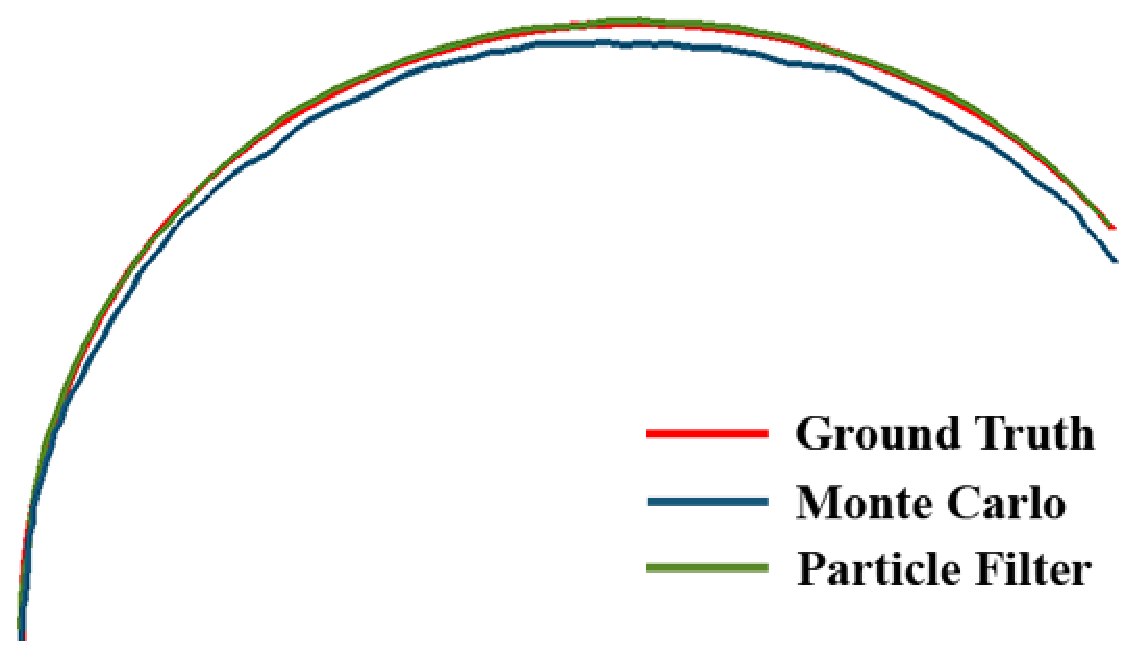
\includegraphics[height=0.5in]{../figures/double_gyre_opt35.eps} }
  \caption{(a): Sampled streamlines computed by the MC method starting from seeding position $x=0.3, y=0.5$ in the analytical double-gyre data set. (b): Sampled streamlines computed by our method from the same seeding position in (a). (c): The most likely traces generated by both methods compared with the ground truth.}
  \label{case_1}
\end{figure}

\subsection{Spatially aggregated Data Sets}

\begin{figure*}[!htbp]
  \centering
  \small
  (a) \vcenterbox{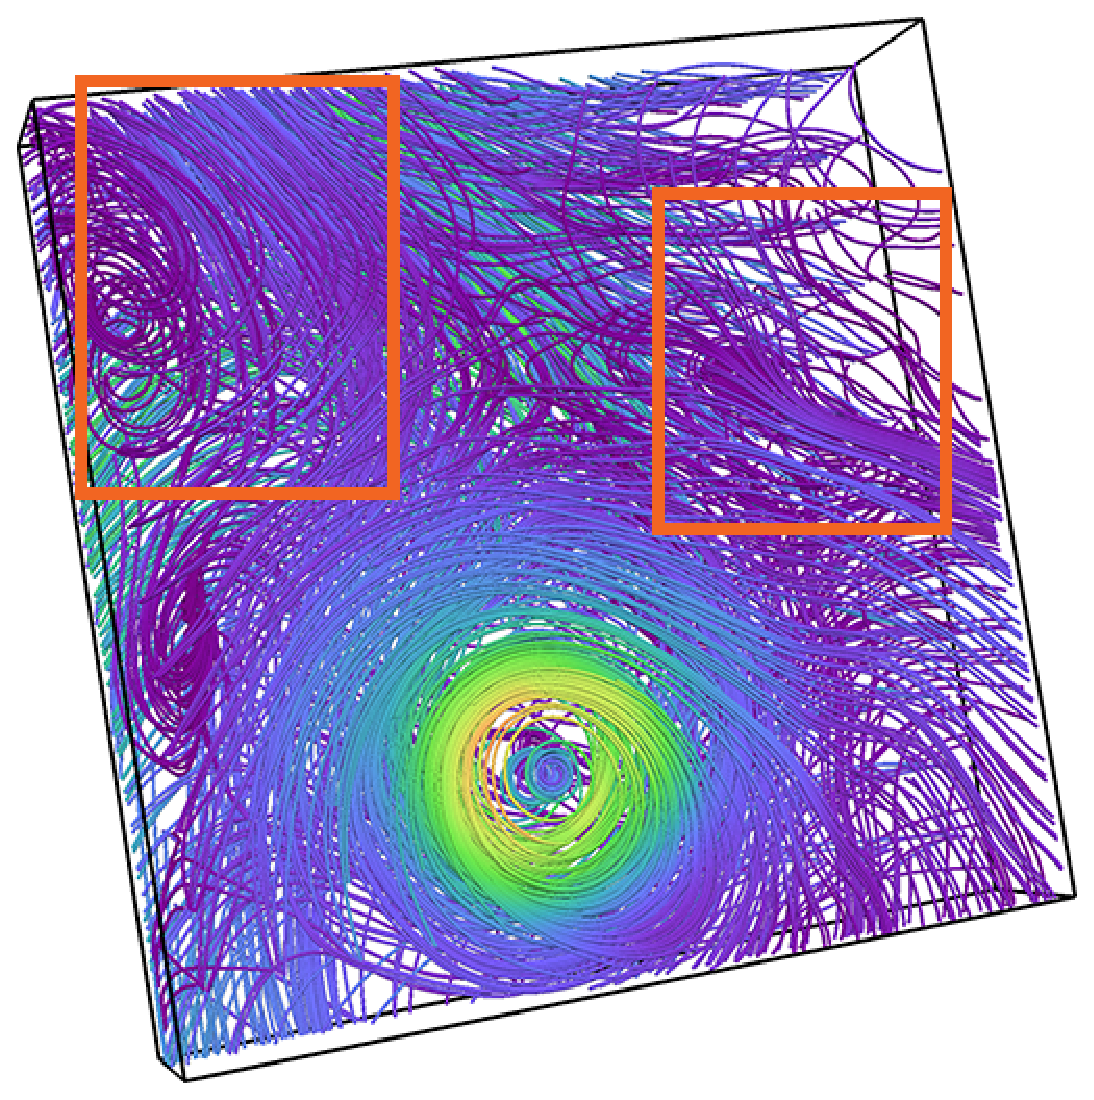
\includegraphics[width=1.5in]{../figures/isabel_gt.eps} } \hfill
  (b) \vcenterbox{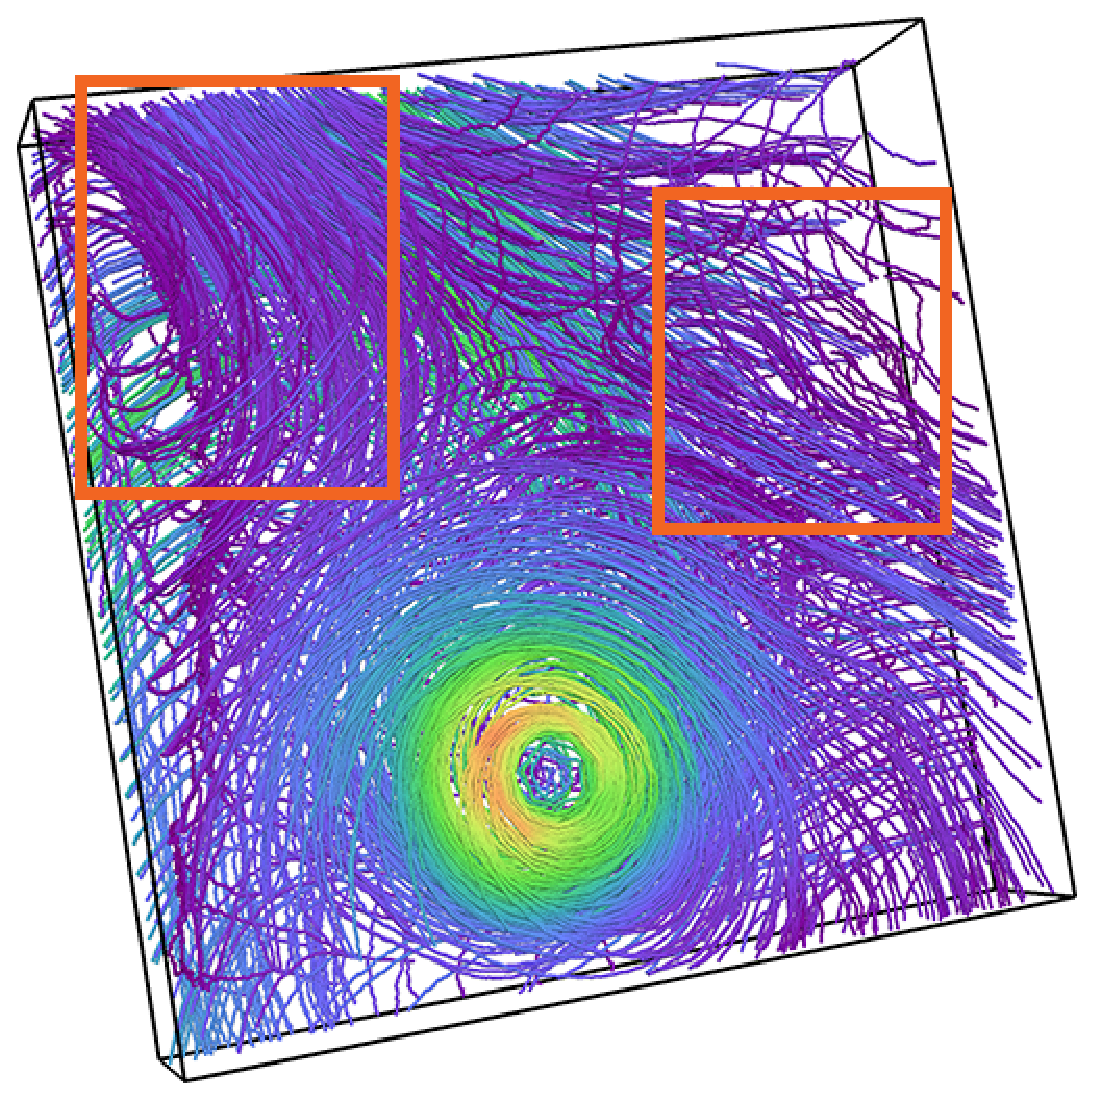
\includegraphics[width=1.5in]{../figures/isabel_mc.eps} } \hfill
  (c) \vcenterbox{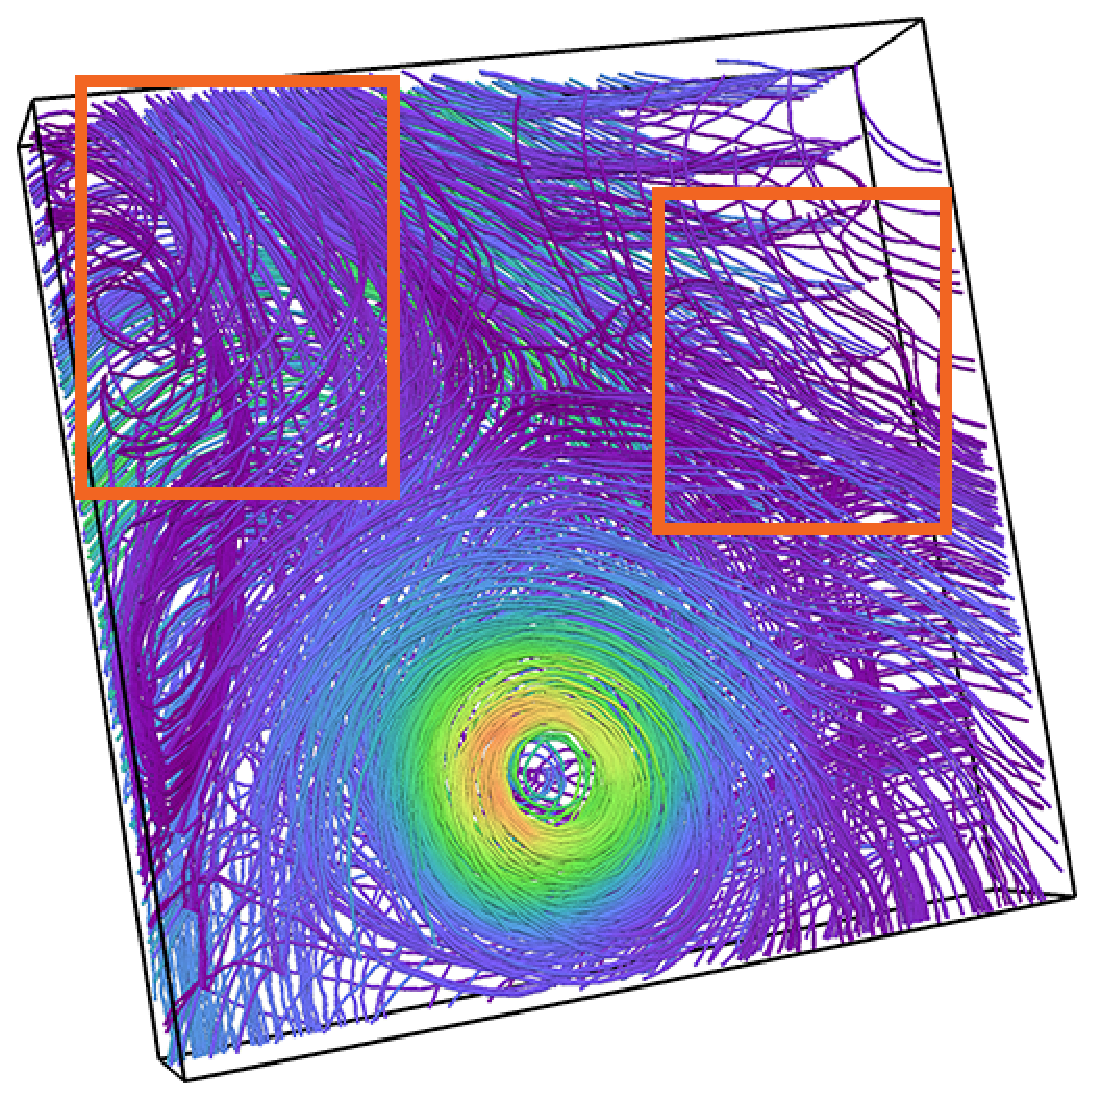
\includegraphics[width=1.5in]{../figures/isabel_smc.eps} }

  \caption{Streamlines generated on the Hurricane Isabel data sets. The color is used to enhance the contrast among streamlines. (a): The ground truth streamlines generated on the raw data. (b): Results produced by the Monte Carlo method on the distribution data with block size $16^3$. (c): Streamlines generated by our method on the same data in (b).}
  \label{data_overview}
\end{figure*}

\begin{figure}[!htbp]
  \centering
  \small
  (a) \vcenterbox{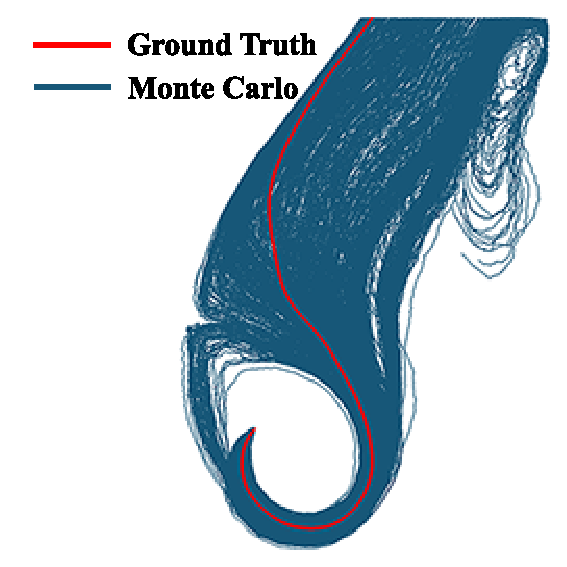
\includegraphics[height=1.0in]{../figures/isabel_mc1.eps} } \hfill
  (b) \vcenterbox{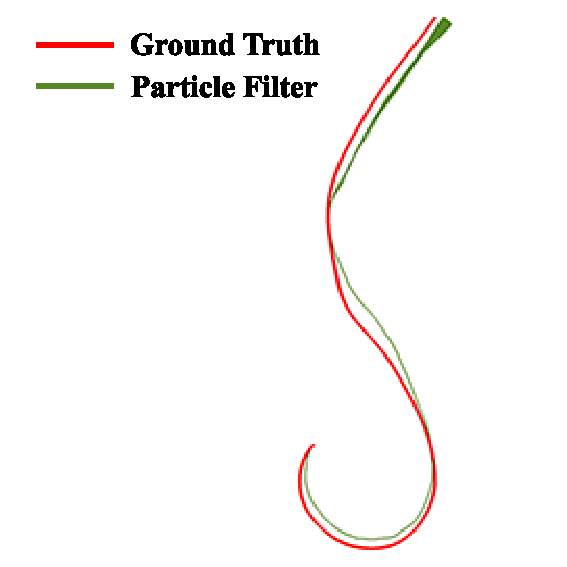
\includegraphics[height=1.0in]{../figures/isabel_smc1.eps} }
  \caption{(a): Sampled streamlines computed by the MC method starting from seeding position $x=250, y=150, z=45$ in the Isabel data set. (b): Sampled streamlines computed by our method from the same seeding position in (a).}
  \label{case_4}
\end{figure}

In this section, experiments were done on the Hurricane Isabel data set. Hurricane Isabel is a data set with a resolution of $500 \times 500 \times 100$ that models a strong hurricane in the west Atlantic region in September 2003. In order to test the performance of our algorithm on uncertain data which represented by non-gaussian distributions, we decompose the data into small cubic blocks and construct a histogram for each block. For the test data set, distribution-based data are generated with three different block size $8^3$, $16^3$, and $32^3$ to evaluate the performance of the proposed algorithm under the influence of uncertainty.

As presented above, we regularly sample a set of seed locations and compute the streamlines for both the raw data and the spatially down sampled data. To perform the quantitative analysis, we treat the streamlines computed from the raw data as the ground truth and compute the distance between the stochastic particle traces with the ground truth. $100$ particles were used with an integration step size $1.0$ and a maximum step number of $1000$ for the streamline computation. Figure~\ref{berror_r} gives the mean of the distances' weighted sum between sample streamline bundles generated from the test methods and the ground truth on the test data set with different block sizes. The figure reveals that the proposed method can produce traces that are closer to the ground truth.

\begin{figure}[!htb]
  \centering
  \begin{subfigure}[b]{0.24\textwidth}
    \centering
    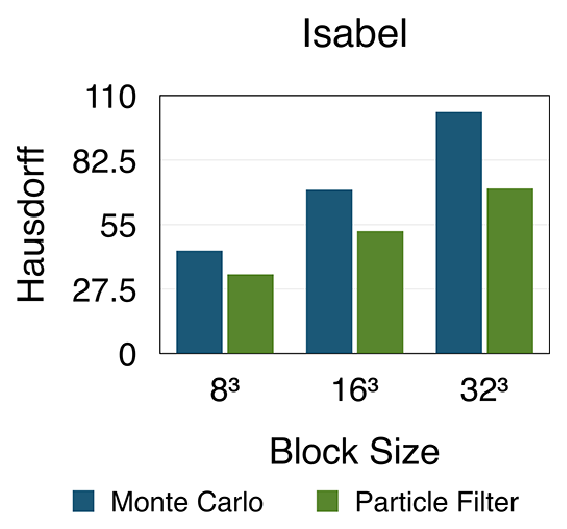
\includegraphics[height=0.9in]{../figures/isabel_h.eps}
  \end{subfigure}~
  \begin{subfigure}[b]{0.24\textwidth}
    \centering
    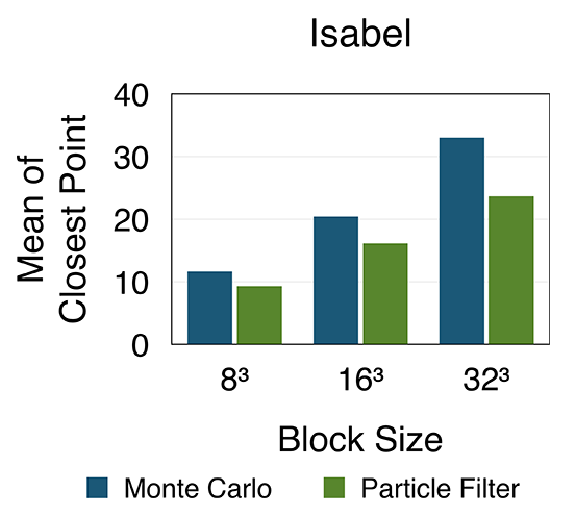
\includegraphics[height=0.9in]{../figures/isabel_m.eps}
  \end{subfigure}
  \caption{Distances between the ground truth and sample traces generated by our method and the MC method for the Isabel data set.}
  \label{berror_r}
\end{figure}

Figure~\ref{data_overview} shows the streamlines generated from the test data set on the seed positions presented above. The most likely streamlines generated by the MC method on the distribution-based data set with block size $16^3$ are given in Figure~\ref{data_overview} (b); as expected, streamlines generated by the MC method are generally not as smooth as the ground truth and some flow features looks quiet different compare with the ground truth. Figure~\ref{data_overview} (c) show the streamlines produced by our method with the same block size, which give more accurate and smoother results. Figure~\ref{case_4} gives sample traces generated by the MC method and the proposed method at a given seed location in the Isabel data set. Figure~\ref{case_4} shows that our algorithm can produce more concentrated and accurate results than the basic MC method, because the correlation between consecutive integration steps are exploited.

\subsection{Performance}

All the experiments were performed on a desktop computer with an Intel(R) Core(TM) i7-4790K CPU 4.0GHz processor, 16GB memory, and an NVIDIA GTX 970 GPU. In Table~\ref{timing}, we compare the performance measurements between the proposed algorithm and the Monte Carlo method for streamlines estimated for a given seed position with $100$ sample points for all the test data sets used in this paper. In all the datasets, our approach is almost as fast as the Monte Carlo method.

\begin{table}[!htb]
\centering
\begin{tabular}{|c|c|c|c|c|}
\hline
\multirow{2}{*}{Data Set}    & \multirow{2}{*}{Method}     & \multicolumn{3}{c|}{Timing(sec)}  \\ \cline{3-5}
                             &                             & 40 Steps  & 80 Steps & 120 Steps  \\ \hline
\multirow{2}{*}{Double Gyre} & MC                          & 0.0026    & 0.005    & 0.008      \\ \cline{2-5}
                             & Bayesian             & 0.0035    & 0.007    & 0.01       \\ \hline
\multirow{2}{*}{Isabel}      & MC                          & 3.3       & 6.7      & 10.1       \\ \cline{2-5}
                             & Bayesian             & 3.4       & 6.8      & 10.7       \\ \hline

\end{tabular}
\caption{Overview of the performance for the proposed algorithm and the Monte Carlo method.}
\label{timing}
\end{table}


\section{Conclusion and Future Work}

In this paper, we present a novel approach for streamline estimation on uncertain steady vector fields. We model the particle tracing problem using a Bayesian framework and solve it using particle filtering. This solution has been tested on two flow field data sets. Compared to the previous methods, our method gives more concentrated traces, and can produce paths of high probability closer to the ground truth.

There are several directions for future research. We will extend our framework to handle time-varying vector datasets, where the specific characteristics of pathlines and streaklines will be taken into account. Secondly, extensions to other flow visualization techniques like FTLE or LIC will be studied.


% %% if specified like this the section will be ommitted in review mode
% \acknowledgements{
% The authors wish to thank A, B, C. This work was supported in part by
% a grant from XYZ.}

\bibliographystyle{abbrv}
%%use following if all content of bibtex file should be shown
%\nocite{*}
\bibliography{draft}
\end{document}
